\documentclass[12pt]{article}
\usepackage[T1]{fontenc}
\usepackage[utf8]{inputenc}
\usepackage{url}
\usepackage{enumerate}
\usepackage[top=3cm, bottom=3cm]{geometry}
\usepackage{graphicx} 
\usepackage{enumitem}
\usepackage{natbib}
\usepackage{listings}
\usepackage{float}
\usepackage{amsmath}
\usepackage{color}
\bibpunct{[}{]}{,}{a}{}{;}
\setcitestyle{super}

% Variables
\newcommand{\assignmentname}{Assignment 1}
\newcommand{\coursename}{Advanced Algorithms and Data Structures}
\newcommand{\studentname}{Bjarki Madsen (lch929) - Michael Bang (tqg432)}
\newcommand{\department}{Department of Computer Science}
\newcommand{\institution}{Copenhagen University}
\newcommand{\location}{Copenhagen, Denmark}

\begin{document}

\renewcommand\refname{References}

\title{\assignmentname \\ {\Large {\textsc \coursename}}}
\author{
        \studentname \\
        \department \\
        \institution \\
        \location
}
\date{\today}

\maketitle
\thispagestyle{empty}

\pagebreak

\section*{Exercise 1}

  Figure \ref{fig:e1_a_solution} shows a b-flow with maximum flow value of 9 for the first proposed graph from the assignment. The second proposed graph from the assignment has no b-flow. The reason is that $v_1$ wants to have at least $3 + c(v_2, v_1)$ after giving away $f(v_1, v_3)$. In order for that to happen the $f(v_2, v_1)$ has to equal to $c(v_2, v_1)$. After the $f(v_2, v_1)$, $v_2$ wants to end up with 1 in demand, meaning it needs a flow value of 4 to itself but that is impossible because the maximum flow to $v_2$ is equal to $c(v_3, v_2)$, or 2 and therefore is unable to fulfill $f(v_2, v_1) = c(v_2, v_1)$. 

  \begin{figure}[h]
    \centering
      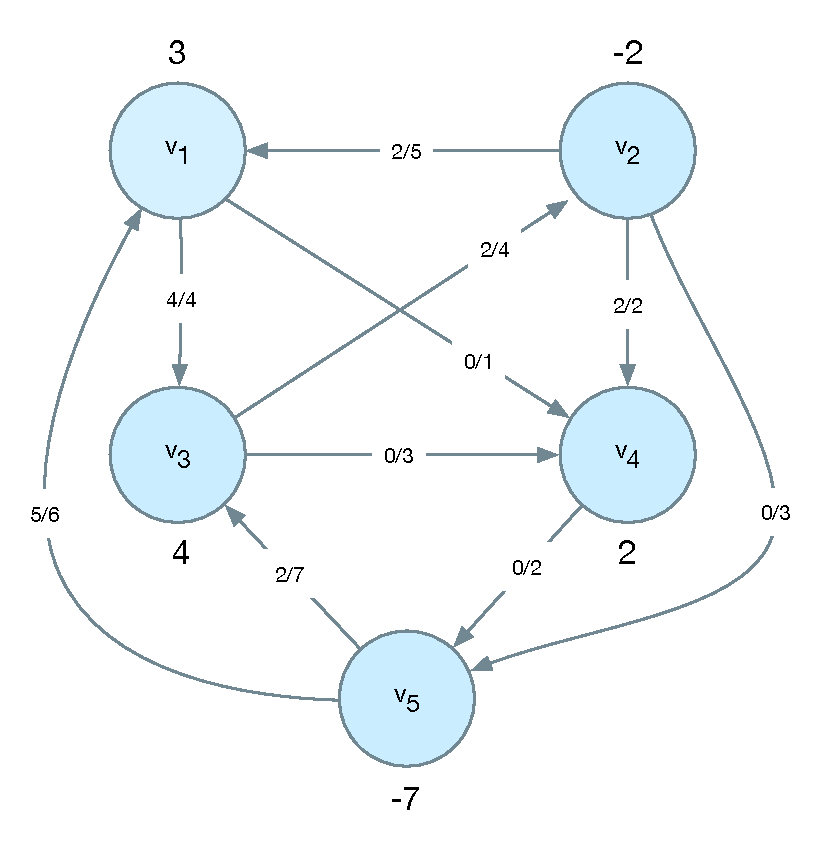
\includegraphics[width=0.6\textwidth]{figures/e1_a_solution}
    \caption{Graph showing b-flow with maximum flow = 9}
    \label{fig:e1_a_solution}
  \end{figure}

\section*{Exercise 2}
\subsection*{Exercise 2.1}

  Tables \ref{table:values_xvf} and \ref{table:values_zfg} show the values for $x_{vf}$ and $z_{fg}$, respectively. The number of breakpoints are 13.
  
  \begin{table}[h]
    \centering
    \begin{tabular}{llllllll}
                                    & \textbf{v1} & \textbf{v2} & \textbf{v3} & \textbf{v4} & \textbf{v5} & \textbf{v6} & \textbf{v7} \\ \cline{2-8} 
    \multicolumn{1}{c|}{\textbf{a}} & 0           & 0           & 1           & 0           & 1           & 1           & 0           \\
    \multicolumn{1}{l|}{\textbf{b}} & 1           & 0           & 0           & 0           & 0           & 1           & 0           \\
    \multicolumn{1}{l|}{\textbf{c}} & 1           & 1           & 1           & 0           & 0           & 0           & 0           \\
    \multicolumn{1}{l|}{\textbf{d}} & 0           & 1           & 1           & -1          & 0           & 1           & 0           \\
    \multicolumn{1}{l|}{\textbf{e}} & 0           & 0           & 1           & 1           & -1          & 1           & 0          
    \end{tabular}
    \caption{The values for $x_{vf}$. For example, $v_1$ has inner turn in the boundary cycle $b$.}
    \label{table:values_xvf}
  \end{table}

  \begin{table}[h]
    \centering
    \begin{tabular}{llllll}
                                    & \textbf{a} & \textbf{b} & \textbf{c} & \textbf{d} & \textbf{e} \\ \cline{2-6} 
    \multicolumn{1}{l|}{\textbf{a}} & 0          & 2          & 1          & 0          & 4          \\
    \multicolumn{1}{l|}{\textbf{b}} & 0          & 0          & 1          & 1          & 0          \\
    \multicolumn{1}{l|}{\textbf{c}} & 0          & 1          & 0          & 0          & 0          \\
    \multicolumn{1}{l|}{\textbf{d}} & 0          & 1          & 0          & 0          & 0          \\
    \multicolumn{1}{l|}{\textbf{e}} & 0          & 0          & 0          & 2          & 0         
    \end{tabular}
    \caption{The values for $z_{fg}$. For example, the number of inner turns between cycle $b$ and $c$ is 1.}
    \label{table:values_zfg}
  \end{table}

\subsection*{Exercise 2.2}
  
  \begin{align*}
      \sum_{f \in F, v \in V}(X_{vf}) + \sum_{f \in F, g \in F}(Z_{fg}-Z_{gf}) = \begin{cases}
                                                                                       4, & \text{if internal}\\
                                                                                      -4, & \text{if external}
                                                                                 \end{cases}
  \end{align*}

\subsection*{Exercise 2.3}
  
  \begin{equation*}
    \begin{aligned}
    & {\text{minimize}}
    & & \sum_{f \in F}\sum_{g \in F \setminus f} z_{fg} \\
    & \text{subject to}
    & & \sum_{f \in F, v \in V}(X_{vf}) + \sum_{f \in F, g \in F}(Z_{fg}-Z_{gf}) = \begin{cases}
                                                                                      4, & \text{if internal}\\
                                                                                      -4, & \text{if external}
                                                                                 \end{cases} \\
    & & & z_{fg} \geq 0
    \end{aligned}
  \end{equation*}


\end{document}
% End of document.







